\subsection{AllTanGenerationTests.java}
AllTanGenerationTests.java is a custom JUnit script to check for vulnerabilities in the Java code of the SCS. It tests for basic validations such as blank or invalid inputs and duplicate TANs.

\subsubsection{InternetBanking}
The test reported 7 failures in the Java code of InternetBanking and passed 1 test successfully See \ref{fig:junit_overview} for the test report.
6 of the failed tests were related to validation of inputs. It was found that the SCS does not perform any validations and generates TAN irrespective of inputs. However, there are some checks on the PHP side, due to which these may be considered as false positives.
However, 1 test \code{shouldNotGenerateDuplicateTan} reveals that the probability of generating duplicate TANs is extremely high and calculated to be \code{13\%}. The number of duplicates were found to be 4 in 100, 232 in 1000, 1222 in 10000 TANs.
Though there is check for duplicate TAN on the PHP side, if frequency of duplicate TANs generated by the SCS is high, the user will have to re-generate TANs multiple times for a successful transfer.

\subsubsection{SecureBank}
The test reported 1 failure in the Java code of SecureBank and passed 7 tests successfully. See \ref{fig:junit_overview_secure_bank} for the test report.
The failed test \code{shouldNotGenerateDuplicateTan} revealed that the probability of duplicate TANs generated is high. However, this is due to the TAN generation logic that generates the same TAN upto 100 seconds. This is done to achieve expiration of the TAN and make it unusable after 100 seconds. Also, this prevents TANs generated at extremely short intervals. Also, after 100 seconds, the probability of duplicate TANs is found to be low. Hence, the test failure can be considered as a false positive.

\begin{figure}[ht]
	\centering
	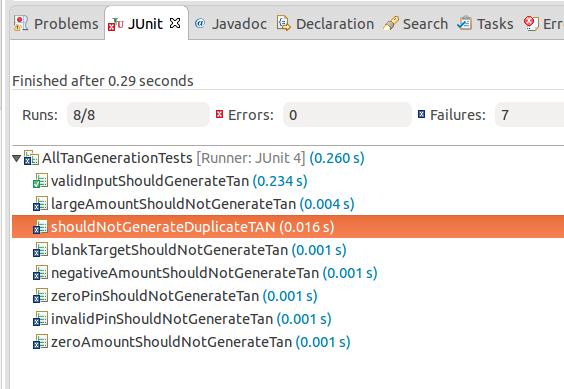
\includegraphics[width=.8\linewidth]{figures/junit_overview.png}
	\caption{Overview of JUnit scan for InternetBanking}
	\label{fig:junit_overview}
\end{figure}

\begin{figure}[ht]
	\centering
	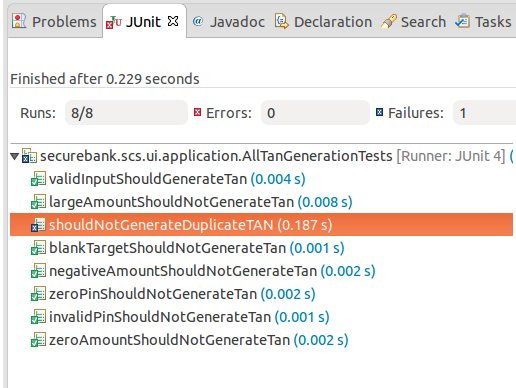
\includegraphics[width=.8\linewidth]{figures/junit_overview_secure_bank.png}
	\caption{Overview of JUnit scan for SecureBank}
	\label{fig:junit_overview_secure_bank}
\end{figure}